So far we have shown how theoretical models influence the data structures
that are available to an entity resolution task.
The question was whether this also has some perceivable outcome in an
experimental setup.
Our experiment proposes using the same entity resolution algorithm across
different data sets to explore whether there are some invariant conditions
that hold true regardless of the data set.

The code for running the experiment is available on GitHub~\cite{matchescu}.
Running the experiment does not require any specific hardware.
We use the Python~\cite{python} programming language (version 3.11) and the
Numpy~\cite{numpy} and Pandas~\cite{pandas2023} libraries for efficient
data manipulation.
All metrics are computed using an OpenSource library available on GitHub as
well~\cite{matchescu-er-metrics2023}.

\subsection{Datasets}\label{subsec:data}

All experiment datasets are available on GitHub\cite{expdata2023}.
These datasets are comprised of three well-known datasets used for
benchmarking entity resolution tasks: Abt-Buy, DBLP-ACM and
Amazon-GoogleProducts~\cite{vldb2010} and a generated dataset~\cite{expdata2023}.
To ease experimentation, we use the original tabular representation
which allows us to take advantage of Pandas~\cite{pandas2010,pandas2023}
and also has the benefit of not requiring adaptation to an internal format.
The tabular data is stored on disk as CSV files.
Each CSV file has a first row containing the column headings and subsequent
rows containing records within which the fields are separated by comma.
The data representation, however, is not important for the experiment's
outcome.

\textcolor{green}{e nevoie sa se argumenteze:\\
1. de ce ai ales aceste 3 seturi de date (de ex pt ca sunt cele mai folosite in literatura)\\
2. de ce ai ales si date reale si data generate, precizand si cum au fost generate aceste date (le putem numi date de control? pt ca de fapt nu sunt generate from scratch, ci e doar o sub-multime a unui dataset real).\\
E nevoie si sa se precizeze dimensiunea aceastor seturi de date (cate exemple sunt, cate features sunt)}

We use the benchmark datasets almost in their original forms and make use
of the ideal mapping to establish the ground truth for each dataset.
The only modification we make to these datasets is shifting the `id' column
to the end.
We make this modification so that algorithms that work on string data are prone
to find more matches.

Conversely, for our custom dataset, we exert complete control over the
entity resolution process.
This is achieved by creating custom input sources for the entity resolution
task through data generation.
These sources use ten chosen items from the `Buy' subset of the
`Abt-Buy' dataset. 
\textcolor{green}{tb spus cum s-au ales cele 10 samples; pur random sau urmarind principii didactice care sa ajute explicatiile}

The data generation procedure divides the ten-item subset into two distinct
tables:

\begin{enumerate}[label=\textbullet,leftmargin=1cm]
\item DG1, with columns: \texttt{`name', `manufacturer', `price', `id'}
\item DG2, with columns: \texttt{`description', `name', `id'}
\end{enumerate}

These tables serve as the foundational input for our experimental analysis.
The construction of the ground truth, as a list of paired elements, is
straightforward due to this data generation approach.
We operate under the assumption that each item in our `Buy' subset
corresponds uniquely to a single real-world entity.
Consequently, the ground truth consists of pairs, each pair representing a
distinct real-world item.

The experiment is set up so that in the data extraction phase that precedes the
actual entity resolution process, the data undergoes uniform conversion to
string format, emphasizing word extraction.
This approach is consistent with both the benchmark and the generated data sets.
The pipeline ensures a left-to-right, top-to-bottom arrangement of extracted
words, with column and row order preservation, thus providing the entity
resolution task references consisting of a single text attribute.
This attribute amalgamates words from all attributes in the source data records
into a cohesive text unit per record.
We employ this process to effectively ensure sequence neutrality.

Let's see how this plays out in practice.
We take the following record from the `Buy' subset as an example.

\begin{table}[ht]
    \setlength\tabcolsep{5pt}
    \begin{tabular}{|l|l|l|l|l|}
        \hline
        id&name&description&manufacturer&price\\
        \hline
        205554724&Seiko SXDA04& & &\$138.00\\
        \hline
    \end{tabular}
    \label{tab:buy-record}
    \caption{An example record of the 'Buy' subset}
\end{table}

The following record is the above data record's corresponding record in DG1. 
\textcolor{green}{I would rephrase the previous statement, avoiding the repetition of "record" word :D. Furthermore, I recommend using the label of the above tabel (above data record -> data record descriebd in Table \ref{tab:buy-record})}


\begin{table}[ht]
    \setlength\tabcolsep{6pt}
    \begin{tabular}{|l|l|l|l|}
        \hline
        name & manufacturer & price & id \\
        \hline
        Seiko SXDA04 & & \$138.00 & 205554724 \\
        \hline
    \end{tabular}
    \label{tab:dg1-record}
    \caption{TBA!}
\end{table}

The corresponding DG2 record would then look as follows.

\begin{table}[ht]
    \setlength\tabcolsep{5pt}
    \begin{tabular}[b]{|l|l|l|}
        \hline
        description&name&id \\
        \hline
        &Seiko SXDA04&205554724 \\
        \hline
    \end{tabular}
    \label{tab:dg2-record}
    \caption{TBA!}
\end{table}

Using the extraction traits described before would yield us the
following entity references from DG1 and DG2, respectively:
\begin{enumerate}
    \item \texttt{(`Seiko',`SXDA04',`\$138.00',`205554724')},
    \item \texttt{(`Seiko',`SXDA04',`205554724')}.
\end{enumerate}

We will refer to our generated dataset with the `mini-buy' moniker.

\subsection{Entity Resolution Algorithm}\label{subsec:entity-resolution-algorithm}

In searching for invariant conditions that hold true regardless of the data set
that we use for experimentation, it is tempting to say that the choice of entity
resolution algorithm is non-consequential.
Given that this experiment is our first foray into the matter, it seems wise not
to give in to temptation.
There are two limitations that we find important in choosing an appropriate
entity resolution algorithm.

Firstly, the algorithm should perform reasonably well without losing the ability
to easily explain its outcome.
In this context we are thinking primarily about quantitative performance marks
such as resource consumption or time spent.

Secondly, we want to choose an algorithm that has very few configurations so
that its qualitative performance is easy to plot over a relatively large  number
of configurations.

The \texttt{ppjoin}\cite{ppjoin} entity matching algorithm meets these criteria.
PPJoin stands for Position Prefix Join.
It is an algorithm designed to find similarities between records by comparing
them using a prefix of each record determined by employing the Jaccard
index~\cite{jaccard1912,finley1996}.
The algorithm's outcomes are intuitively easy to explain.
A lower Jaccard threshold will cause the algorithm to take into account shorter
prefixes, thus increasing the chances of a match.
A higher threshold should match fewer items, but with less chance for error.
Throughout the experiment, the Jaccard threshold will be denoted with \textit{t}.

Our experiment consists of the following steps:

\begin{itemize}
    \item generate or load the data;
    \item take 100 entity matching passes through the input data with
          Jaccard thresholds ranging from 0 to and including 0.99 in steps of
          0.01, storing the results for each step;
    \item compute the statistical and algebraic similarity metrics for each
          of the stored results.
\end{itemize}

The \texttt{ppjoin} algorithm treats entity resolution as a matching problem.
Consequently, the mathematical model that fits it very well is the statistical
model.
From this it follows that 
\textcolor{green}{I would replace "from this it follows that" by "Hence" / "Therefore" / "accordingly" / "consequently"} 
in order to evaluate the quality of the algorithm
under the algebraic model, we have to convert a list of matches (which is what
\texttt{ppjoin} outputs) to a partition over a set.

For our own generated data we are able to generate the ground truth partition
for the algebraic model based on the input data.
For the benchmark data sets we convert the ideal mapping to a partition over the
input data using the Union-Find data structure and a simplified version of
Kruskal's algorithm.

\subsection{Outcomes from Generated Data}\label{subsec:experiment-mini-buy}

\subsubsection{Statistical Results}

The ground truth and the results are represented as lists of pairs.
The ground truth was generated by iterating over both input data sources using
the same cursor and outputting pairs of records.
Note that there are duplicate CSV records that only differ on the `id' column.

Intuition tells us that for values of the Jaccard similarity threshold
\textit{t}\footnote[1]{the Jaccard similarity coefficient is used to determine
the length of the prefix which should be used to compare two entity references
to determine whether they refer to the same entity or not} that are either too
low or too high we should have lower precision.
For higher thresholds we should also have lower recall values, whereas for
lower values the recall should be higher.
Figure~\ref{fig:mini-buy-fs} shows the \texttt{ppjoin} results at various
values of the Jaccard threshold $t$.


\textcolor{green}{please check this paper \href{https://hpi.de/fileadmin/user_upload/fachgebiete/naumann/publications/2013/On_Choosing_Thresholds_for_Duplicate_Detection.pdf}{link}, also - because it disscuss about a particular effect of dataset size in entity resolution in the context of choosing similarity thresholds. }
\begin{figure}[!hp]
    \centering
    \captionsetup{justification=centering}
    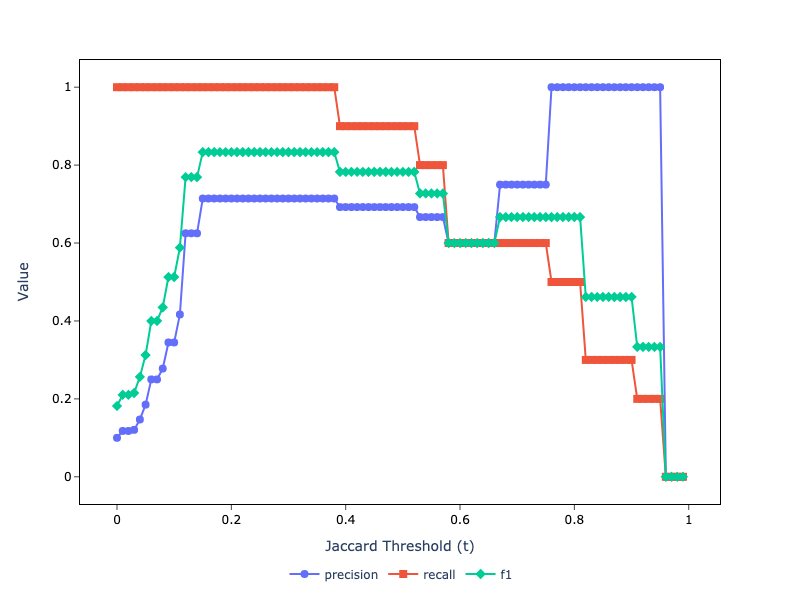
\includegraphics[width=\columnwidth]{mini-buy-fsm-main}
    \caption{Statistical metrics on `mini-buy' dataset
    \textcolor{green}{for results of F-S model}
    }
    \label{fig:mini-buy-fs}
\end{figure}

We can make some observations based on Figure~\ref{fig:mini-buy-fs}.
For values of $t \geq 0.78$, we end up with fewer, but more accurate matches.
\textcolor{green}{fewer = ?; daca P creste si R scade, inseamna ca FP scade si FN creste...nu?} 
For values of $0.36 \leq t \leq 0.6$, both precision and recall increase. 
\textcolor{green}{pe figura, in acest interval si P  si R scad. Oare de ce zici ca ele cresc?} 
Our intuition tells us that precision should decrease as \textit{t} decreases,
but that is not the case.
\textcolor{green}{dar pe (0,0.2) P scade! asa cum zice urm propoz!} 
When $t$ is nearing zero, recall is maximal while precision decreases towards
zero.

The generated data set contains items such as those with the IDs
\texttt{208114672} and \texttt{208114673} which are near-identical.
For lower values of \textit{t}, the algorithm produces two true positives and
two false positives.
By itself, this change 
\textcolor{green}{Which one?} 
should lower the precision.
Lower values of \textit{t} also broaden the spectrum of what is available for
comparison (e.g~items with shorter names, like \texttt{205554724}).
By having new items to compare, we also increase the amount of true positives.
This dynamic ends up increasing precision as we lower values of \textit{t} so
long as we are not operating on the full input set.

Note that while we do describe the dynamic specifically for the \texttt{ppjoin}
algorithm, the dynamic itself is not algorithm specific at all.
Regardless of the algorithm that we use, given some specific circumstances it is
possible to obtain the same dynamic which results in increasing precision
contrary to our intuition.
This is interesting because by influencing the value of the F1 score, it also
determines the observer's perception of what input configuration they should use
should they want a balanced output from the entity resolution task. 
\textcolor{green}{e cam incalcita exprimarea; oare nu se potae reformula? in plus, as avea grija la folosirea "this" si "that"; e mai clar daca au si substantive langa ele; in fraza de mai sus, de ex. this is interesting -> this hypothesis / assumption is interesting} 
In our example, we should aim for a value of $0.15\leq t \leq 0.38$ \textcolor{green}{in order to ???}.

On the other hand, balance 
\textcolor{green}{of P and R? or "trade-off of P and R"} 
might not be at all what we are looking for.
We see that perfect recall is achieved with $t \leq 0.38$ and perfect precision
is achieved with $0.76 \leq t \leq 0.95$.
These values are still useful in certain domains where entity resolution is
prominently applied.
For instance, a core legal principle applicable in many jurisdictions across the
world states that is far more favourable to let 100 guilty people escape than to
put one innocent behind bars.
By that logic, we only care about precision.
Perfect recall while still retaining some precision might be useful during
research (works on the same topic) or medical diagnosis (other cases with the same
symptoms).
In these cases, sifting through false positives might be preferable to missing
out on important information because of a false negative that is due to a
suboptimal input configuration.

\subsubsection{Pairwise Metrics}

The ground truth and the result of the ER process are represented as partitions
over an input set of data.
Because we include the IDs in both DG1 and DG2, the input data set will
contain 20 items.
The ground truth contains 10 pairs of items.

Measuring the similarity of two partitions can be accomplished in more ways than
measuring the statistical success of a matching process.
Among these metrics, the pairwise comparison of two partitions is the best
approximation of the statistical metrics\cite{Men10}.
Figure~\ref{fig:mini-alg-pairwise} shows the computed pairwise metrics for
various values of \textit{t}.

\begin{figure}[!h]
    \centering
    \captionsetup{justification=centering}
    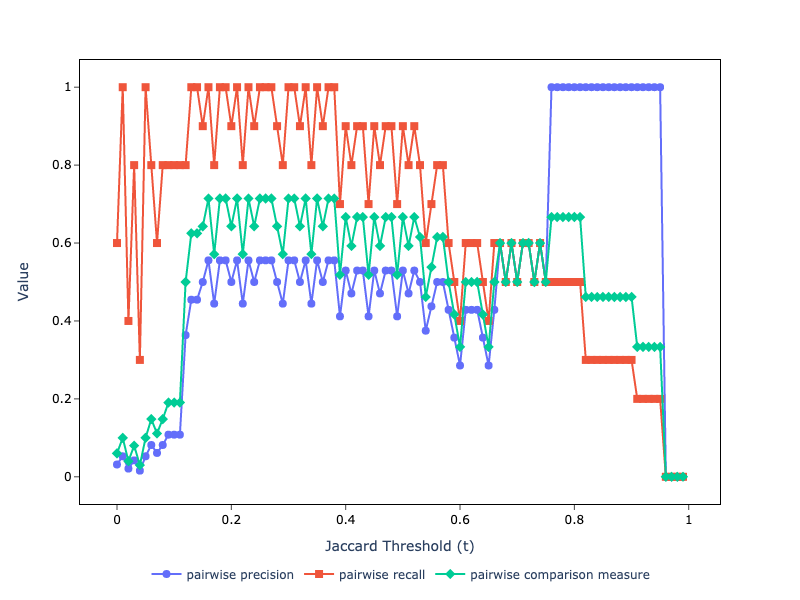
\includegraphics[width=\columnwidth]{mini-buy-algebraic-pairwise}
    \caption{Pairwise metrics on `mini-buy' dataset
    \textcolor{green}{for results of algebric model}\\
    \textcolor{green}{oare in legenda, la verde, nu ar tb sa fie pairwise F1?}
    }
    \label{fig:mini-alg-pairwise}
\end{figure}

We can see a plot similar to the one in Figure~\ref{fig:mini-buy-fs}.
The optimal range for high PF1 scores is the same to the case of statistical measures and the pairwise precision plot's shape
is almost identical (save for a smoother in the statistical model).

It is in terms of recall where we see a major difference from the statistical
model's plot.
More specifically, for $t \le 0.12$ pairwise recall drops significantly whereas
statistical recall stays at the maximum value.
The reason behind this variation lies in the difference between the two models of entity
resolution.
Whereas the standard recall formula only accounts for false negatives (of which
we can not have any using the generated data set), pairwise recall requires the
result data to be partitioned.
The partitioning operation removes any duplicates a partition class might
contain (such as duplicate matches returned by \texttt{ppjoin} for very low
values of \textit{t}).
This means that statistical recall simply does not account for the situation
when the entity resolution algorithm returns extremely large amounts of data
that also happen to contain all the true positives in the ground truth.

We note again that while the circumstances in which we show this behaviour are
specific to \texttt{ppjoin}, the phenomenon in itself is specific to the model
we employ when we evaluate the algorithm's performance.
Other algorithms may provide the conditions for this phenomenon using their own
input configurations.
To ensure a valid measurement system (one that is both accurate and precise), we
should collect pairwise metrics along with statistical metrics.

\subsubsection{Cluster Metrics}

Pairwise metrics are a form of measuring how well-formed the output of an entity
resolution task is.
The other widely spread family of metrics from this category that resembles
statistical metrics are the cluster metrics, which are displayed in
Figure~\ref{fig:mini-alg-cluster} for 'mini-buy' dataset.

\begin{figure}[!h]
    \centering
    \captionsetup{justification=centering}
    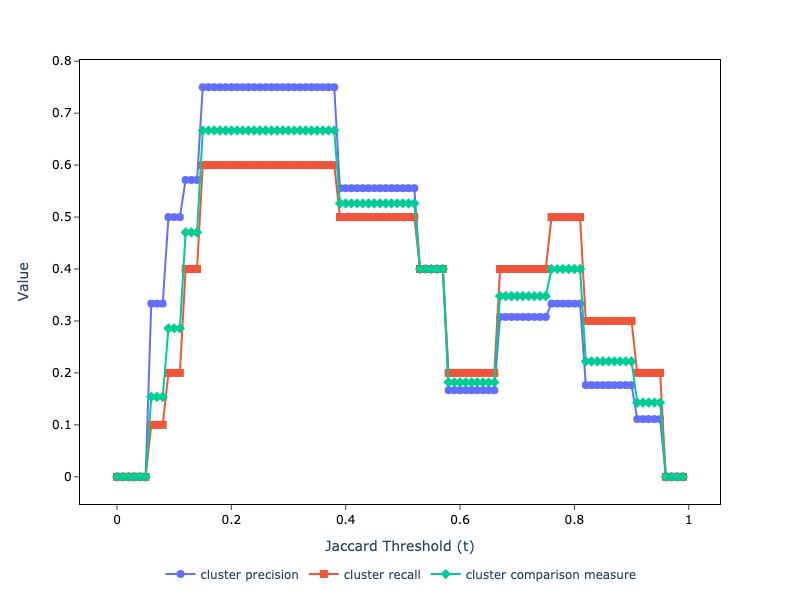
\includegraphics[width=\columnwidth]{mini-buy-algebraic-cluster}
    \caption{Cluster metrics on `mini-buy' dataset 
    \textcolor{green}{for results of algebric model}\\
    \textcolor{green}{oare in legenda, la verde, nu ar tb sa fie cluster F1? (stiu ca e sisnonim cu CCM, dar cand s-a dat formula a fost botezata CF1, iar in prima figura s-a facut referire tot la F1)}
    }
    \label{fig:mini-alg-cluster}
\end{figure}

It is refreshing to see that the optimal value of \textit{t} for a well-balanced
output should still be in the $\left[0.15,0.38\right]$ interval.
We also notice that cluster metrics point out the lack of recall when \textit{t}
nears zero even more than the pairwise metrics.
A more nuanced point is that recall decreases for $t \in \left[0.38,0.58\right]$
much more pronouncedly.

Clustering metrics also reveal interesting aspects about the other metrics we have
seen so far.
For example, we expect increased statistical and pairwise precision to
correspond to increased cluster precision.
This is only somewhat true.
As \textit{t} decreases, we see statistical and pairwise precision increasing
along with cluster precision.
What is interesting is just how much cluster precision increases.
As \textit{t} decreases, more and larger clusters are returned by the entity
resolution task.
For a series of values of \textit{t} the number of returned clusters does not
change much, while the shape of the partition returned by the entity resolution
task becomes more and more similar to the shape of the ground truth.
As the entity resolution task starts returning larger and larger clusters, the
cluster precision drops significantly even though the number of clusters
returned by the entity resolution task drops as well.

A similar effect can be observed for cluster recall as we increase the value of
\textit{t}.
When statistical precision increases, there is a good chance that the number of
clusters in the entity resolution result which are in agreement with the ground
truth would also increase.
Because there are fewer matches as statistical precision increases, we have a
partition that contains many singletons.
This causes cluster precision to decrease (because it relates to the number of
clusters returned by the entity resolution task) and cluster recall to increase
(because it relates to the number of clusters in the ground truth which remains
constant).

These phenomena do not depend on the entity resolution algorithm, but are
characteristics of cluster precision and cluster recall.
Higher statistical recall will always mean fewer and larger clusters some of
which will overlap with clusters in the ground truth.
Higher statistical precision will always mean more singleton clusters returned
by the entity resolution task which, in turn, will increase cluster recall.

Remembering that we might not care about balanced output, we can consider
cluster precision and cluster recall as metrics that balance out the bias built
into statistical precision and recall.
Furthermore, cluster precision and recall can also be used together with
pairwise metrics to confirm any blind spots in the statistical metrics.

In our own practical example, we will use these findings to keep an eye on
$t\in\left[0.76,0.81\right]$ as an interesting input configuration when we are
biased towards better precision.

\subsubsection{Clustering Indexes}

Even though pairwise and cluster metrics complement the statistical metrics,
sometimes all we want is a clear picture of the optimal input configurations for
the algorithm.
The easiest way to glean this information is by using one of the clustering
indexes depicted in Figure~\ref{fig:mini-alg}.

\begin{figure}[!h]
    \centering
    \captionsetup{justification=centering}
    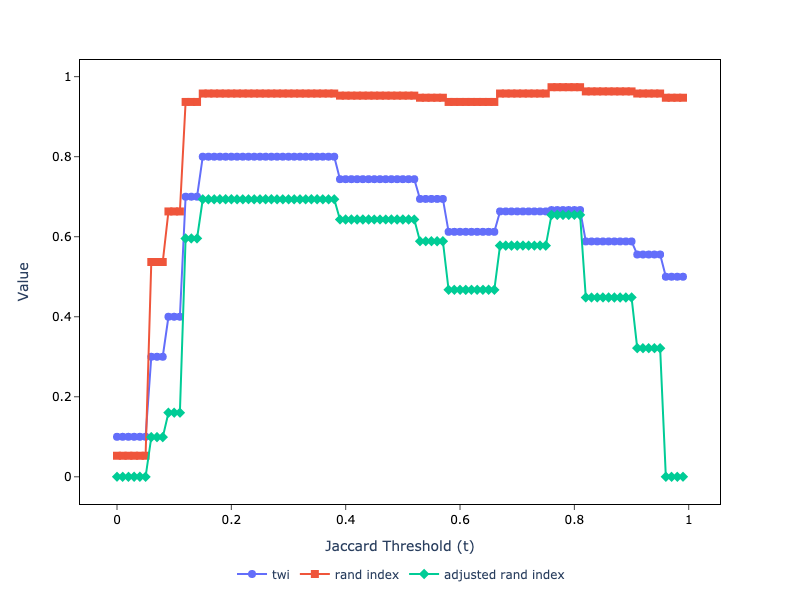
\includegraphics[width=\columnwidth]{mini-buy-algebraic-main}
    \caption{Clustering indexes on `mini-buy' dataset}
    \label{fig:mini-alg}
\end{figure}

We observe that the plot of the Adjusted Rand Index indicates both the desirable
and the undesirable values of \textit{t}.
Notice that it ranks $t\in\left[0.76,0.81\right]$ almost as highly as
$t\in\left[0.15,0.38\right]$.
By following its plot, we should stay clear of values of \textit{t} from other
intervals --- especially those at the extremities of the definition interval.

By comparison with the ARI, the Rand Index itself is not very informative.
It signals that recall is not perfect for values of \textit{t} nearing zero and
does give the highest score for $t\in\left[0.76,0.81\right]$.
However, it also gives high scores for values of \textit{t} where all the other
metrics do not.

The Talburt-Wang index's plot is a fairly good indicator, taking all our former
observations into account.
The only aspect where it is lagging is for $t\in\left[0.76,0.81\right]$.
Here it fails to clarify the favorable circumstances due to high statistical
precision and high cluster recall.

Based on these observations, we can only echo the existing literature 
\textcolor{green}{please add a ref!}
.
The Adjusted Rand Index or, if operational performance is key, the Talburt-Wang
Index provide enough meaningful information to find the ballpark of the ideal
configuration settings for an entity resolution task.

\subsection{Outcomes from Benchmark Datasets}\label{subsec:experiment-benchmark}

So far we have seen evidence on the generated miniature dataset that each
theoretical model provides a lens through which we can interpret various aspects
of an entity resolution task's qualitative performance.
Some invariants with respect to the entity resolution task have been discovered.
Nothing related to the task that is being evaluated determines these phenomena.
However, we don't know if any of them are invariant with respect to the data
being used.

We want to understand if there are conditions or phenomena that could help us
extract universally good input configurations for an entity resolution algorithm
by using a small dataset.
There already seem to exist some interesting relationships between metrics
including a blind spot in how statistical recall is computed regardless of the
used entity resolution algorithm.
Now we have to see if any of them persist if we change the data used for
performing entity resolution.

In order to do this we shall use benchmark datasets.
The first of these is the `Abt-Buy' data set~\cite{vldb2010} and the plots for
our experiment are available in Figures~\ref{fig:abt-buy-fsm-main},
~\ref{fig:abt-buy-algebraic-pairwise},~\ref{fig:abt-buy-algebraic-cluster}
and~\ref{fig:abt-buy-algebraic-main}.

\begin{figure*}[ht]
    \begin{minipage}{0.24\textwidth}
        \centering
        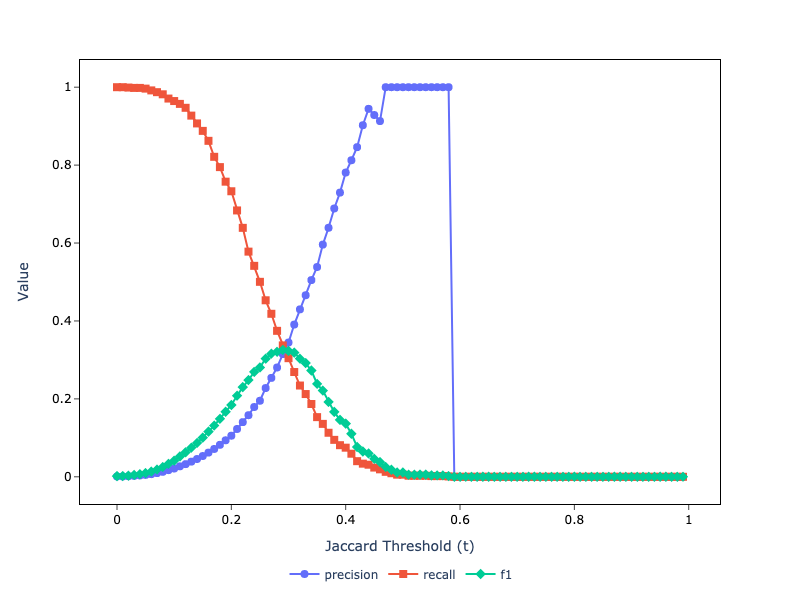
\includegraphics[width=\textwidth]{abt-buy-fsm-main}
        \caption{Abt-Buy statistical metrics.}
        \label{fig:abt-buy-fsm-main}
    \end{minipage}
    \begin{minipage}{0.24\textwidth}
        \centering
        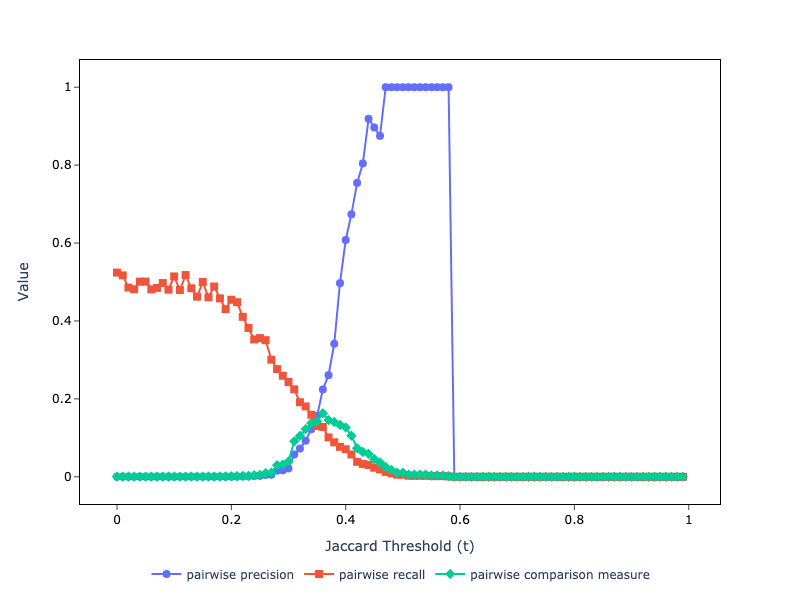
\includegraphics[width=\textwidth]{abt-buy-algebraic-pairwise}
        \caption{Abt-Buy pairwise metrics.}
        \label{fig:abt-buy-algebraic-pairwise}
    \end{minipage}
    \begin{minipage}{0.24\textwidth}
        \centering
        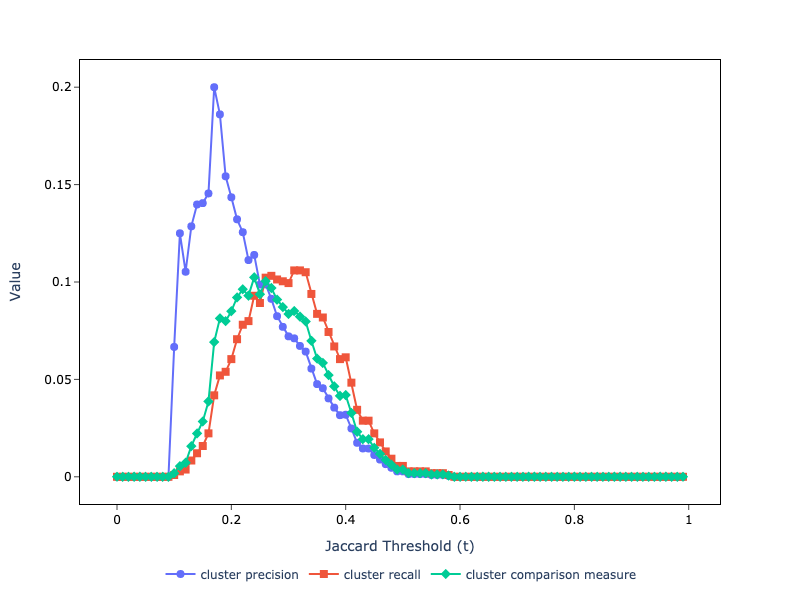
\includegraphics[width=\textwidth]{abt-buy-algebraic-cluster}
        \caption{Abt-Buy cluster metrics.}
        \label{fig:abt-buy-algebraic-cluster}
    \end{minipage}
    \begin{minipage}{0.24\textwidth}
        \centering
        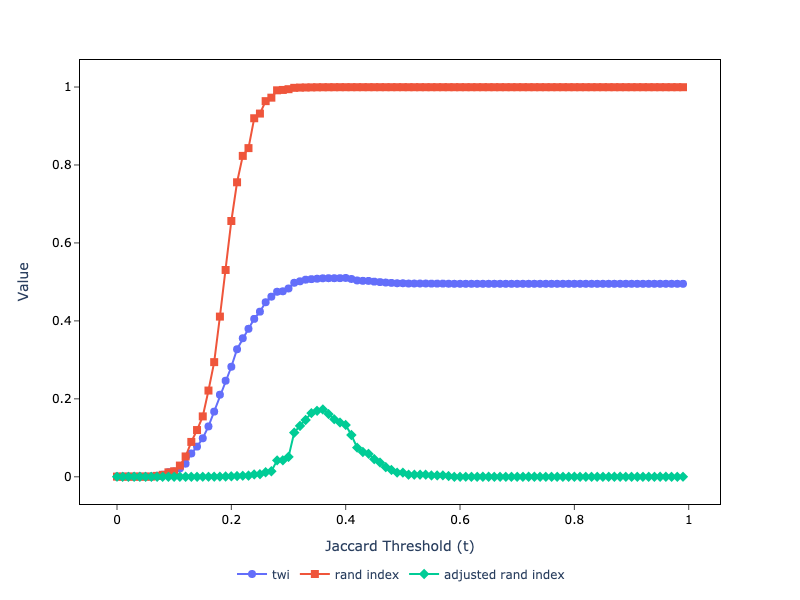
\includegraphics[width=\textwidth]{abt-buy-algebraic-main}
        \caption{Abt-Buy clustering indexes.}
        \label{fig:abt-buy-algebraic-main}
    \end{minipage}
\end{figure*}\label{abt-buy}

We can see that the statistical model still has a pronounced bias towards higher
recall values.
The other invariant that also seems to hold for this dataset as well is the
balancing/confirmation action of the cluster metrics with respect to the
statistical/pairwise metrics.
Another nice confirmation is that the pairwise recall is never perfect.
Lastly, the clustering indexes are good approximates of the ballpark where
we could find  interesting input configurations.
All interesting values of \textit{t} 
\textcolor{green}{I would indicate the value or the value's range for this optimal $t$} 
are in the ballpark indicated by these
indexes.

On the other hand, we can clearly see that input configurations 
\textcolor{green}{la ce anume te referi prin aceste "input configs"? Ai mai amintit si mai devreme, dar nicaieri nu e specifica clar la ce anume se refera; e vorba doar de pagrul $t$ sau si de algoritm de ER si alti params?}  
such as those
that take advantage of a high precision to high cluster recall correlation are
dataset specific.

We move on to the `Amazon-Google Products' data set~\cite{vldb2010} and observe
the results in Figures~\ref{fig:amazon-googleproducts-fsm-main},
\ref{fig:amazon-googleproducts-algebraic-pairwise},
\ref{fig:amazon-googleproducts-algebraic-cluster} and
\ref{fig:amazon-googleproducts-algebraic-main}.

\begin{figure*}[h]
    \begin{minipage}{0.24\textwidth}
        \centering
        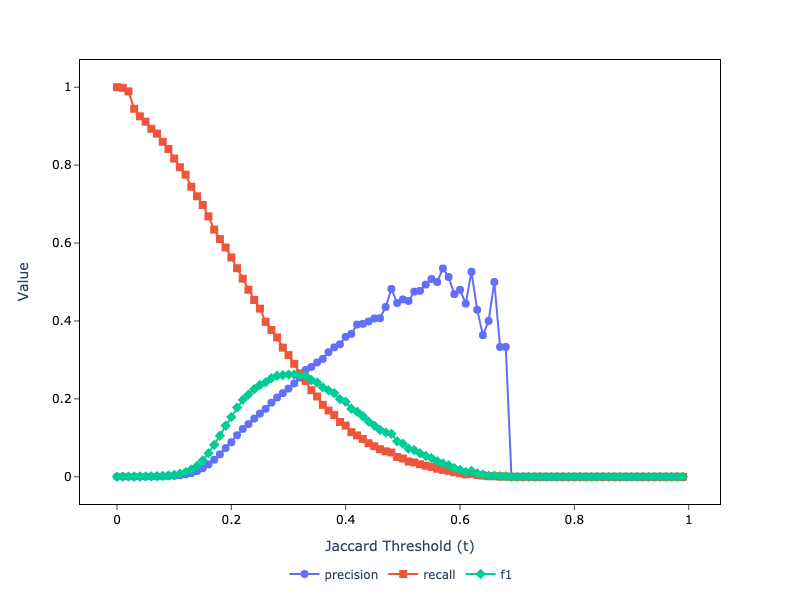
\includegraphics[width=\textwidth]{amazon-googleproducts-fsm-main}
        \caption{Amazon-Google statistical metrics.}
        \label{fig:amazon-googleproducts-fsm-main}
    \end{minipage}
    \begin{minipage}{0.24\textwidth}
        \centering
        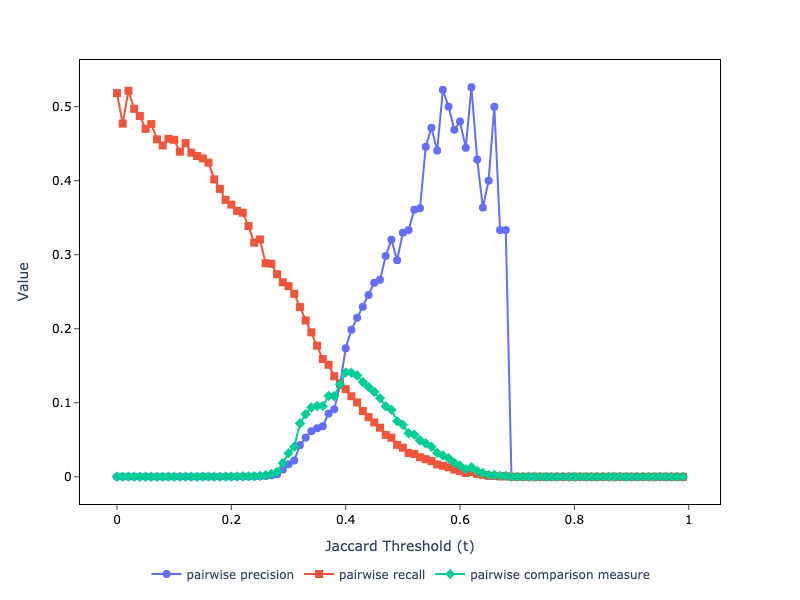
\includegraphics[width=\textwidth]{amazon-googleproducts-algebraic-pairwise}
        \caption{Amazon-Google pairwise metrics.}
        \label{fig:amazon-googleproducts-algebraic-pairwise}
    \end{minipage}
    \begin{minipage}{0.24\textwidth}
        \centering
        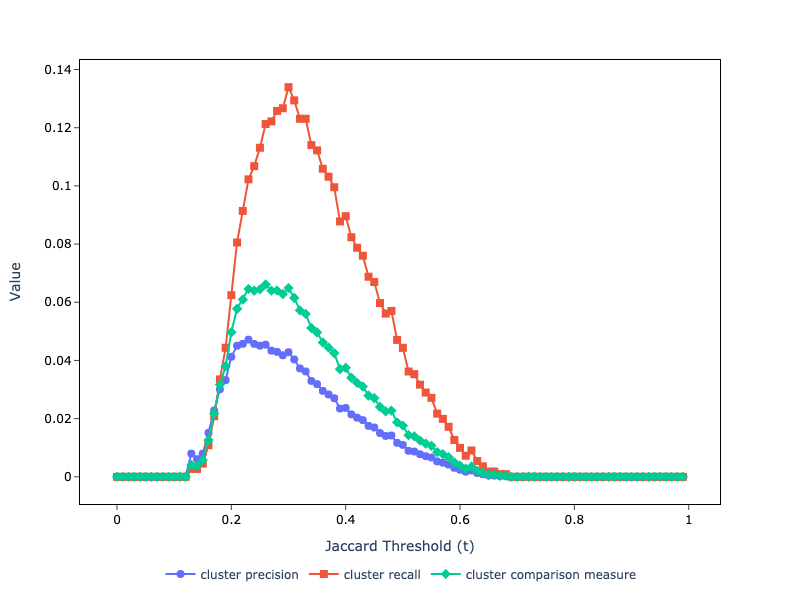
\includegraphics[width=\textwidth]{amazon-googleproducts-algebraic-cluster}
        \caption{Amazon-Google cluster metrics.}
        \label{fig:amazon-googleproducts-algebraic-cluster}
    \end{minipage}
    \begin{minipage}{0.24\textwidth}
        \centering
        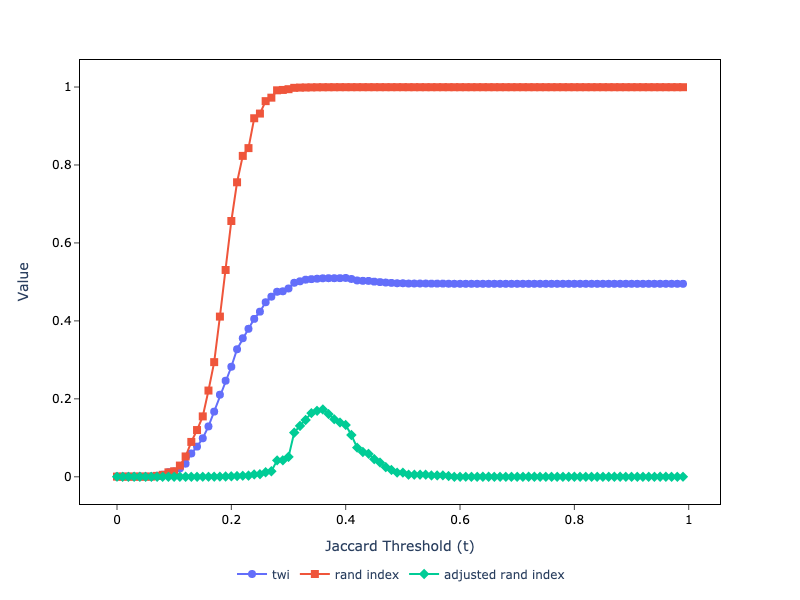
\includegraphics[width=\textwidth]{abt-buy-algebraic-main}
        \caption{Amazon-Google clustering indexes.}
        \label{fig:amazon-googleproducts-algebraic-main}
    \end{minipage}
\end{figure*}\label{amazon-google}

The plotted data shows that the statistical model is biased toward high recall
in this data set, also.
It also shows that pairwise metrics show lower score for recall while
maintaining the shape of the plot for statistical metrics.
Albeit less clearly, we still see that cluster precision and cluster recall can
still act as a balancing weight or confirmation for the statistical metrics or
pairwise metrics, respectively.

On the other hand, we start seeing that the clustering indexes are no longer
individually indicating a ballpark correctly.
The Talburt-Wang index seems to indicate the same optimal input configuration as
the cluster metrics, whereas the Adjusted Rand Index seems to provide a ballpark
of optimal input configurations that would also maximize scores obtained for
pairwise metrics and statistical metrics.
Even though one can assume that this is because of how the two indexes are
defined (TWI counts agreements on whole clusters while ARI counts agreeing
pairs), confirming this assumption experimentally requires further work.
Regardless, we can safely conclude that whether clustering indexes reveal
ballparks for optimal input configurations is dataset dependent.
\textcolor{green}{mie nu mi-e clar ce ai vrut sa spui :(}

Finally, we look at the `DBLP-ACM' benchmark dataset~\cite{vldb2010}.
The plots we obtained after running the experiment on this dataset are available
in Figures~\ref{fig:dblp2-acm-fsm-main},
\ref{fig:dblp2-acm-algebraic-pairwise},
\ref{fig:dblp2-acm-algebraic-cluster} and
\ref{fig:dblp2-acm-algebraic-main}.

\begin{figure*}[h]
    \begin{minipage}{0.24\textwidth}
        \centering
        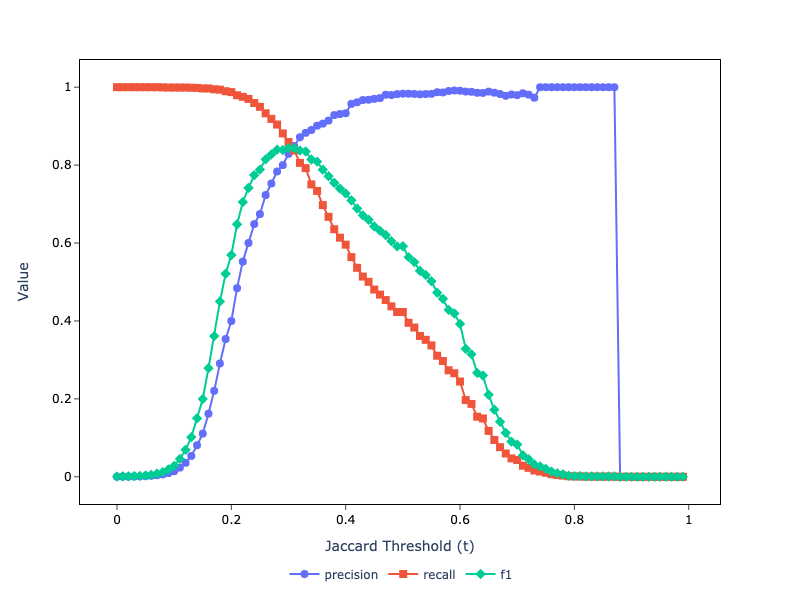
\includegraphics[width=\textwidth]{dblp2-acm-fsm-main}
        \caption{DBLP-ACM statistical metrics.}
        \label{fig:dblp2-acm-fsm-main}
    \end{minipage}
    \begin{minipage}{0.24\textwidth}
        \centering
        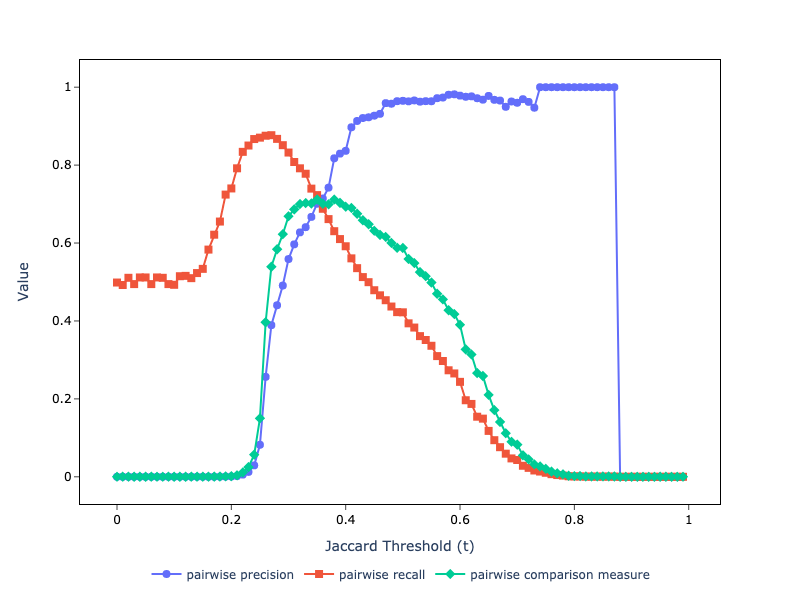
\includegraphics[width=\textwidth]{dblp2-acm-algebraic-pairwise}
        \caption{DBLP-ACM pairwise metrics.}
        \label{fig:dblp2-acm-algebraic-pairwise}
    \end{minipage}
    \begin{minipage}{0.24\textwidth}
        \centering
        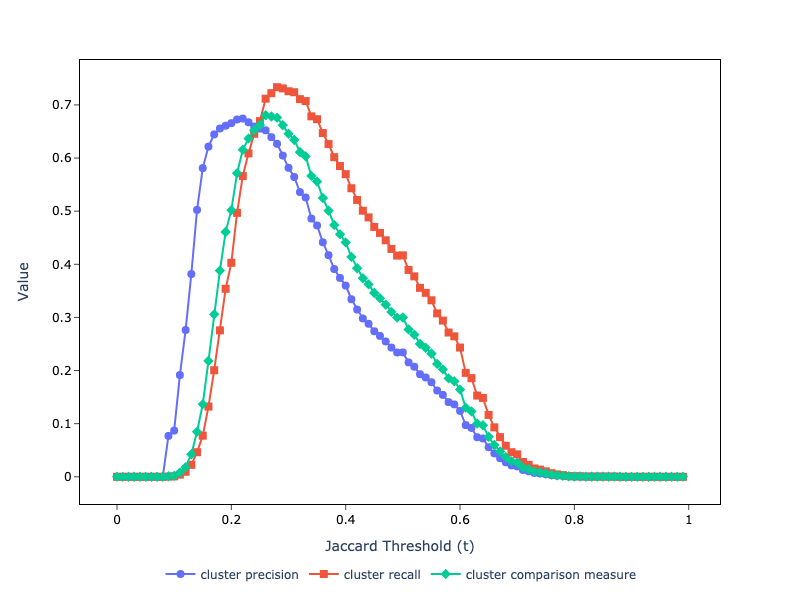
\includegraphics[width=\textwidth]{dblp2-acm-algebraic-cluster}
        \caption{DBLP-ACM cluster metrics.}
        \label{fig:dblp2-acm-algebraic-cluster}
    \end{minipage}
    \begin{minipage}{0.24\textwidth}
        \centering
        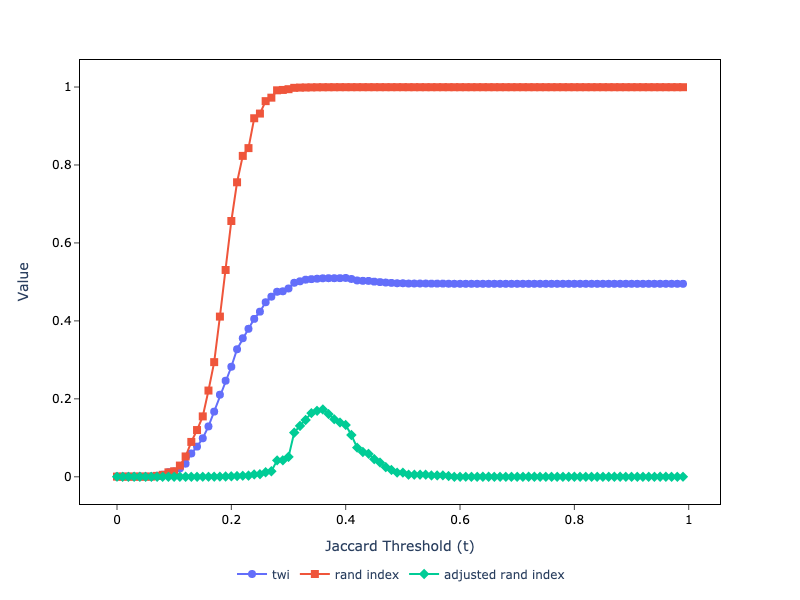
\includegraphics[width=\textwidth]{abt-buy-algebraic-main}
        \caption{DBLP-ACM clustering indexes.}
        \label{fig:dblp2-acm-algebraic-main}
    \end{minipage}
\end{figure*}\label{dblp2-acm}

Looking at the plots for this last dataset we again see confirmation that recall
in the statistical model is much higher than advertised by any of the other
metrics.
The other condition that is invariant with respect to the algorithm and the
data sets is that cluster precision and cluster recall act as good balancing or
confirmation metrics for the statistical and pairwise metrics, respectively.
\textcolor{green}{mie nu mi-e clar ce ai vrut sa spui :(}

We also see that the conjecture concerning the TWI as a good approximation for
input configurations that yield high clustering scores holds for this data set,
too. 
The same can be said about the ARI for approximating high scores with regard to
matching.
These observations hold for all four datasets we have experimented on.


\textcolor{green}{As incerca sa le enunt din nou acest concluzii, iar dupa ce sunt formulate le-as transforma in ipoteze, descriindu-le la inceputul sectiunii cu experimentele; astfel, ele vor reprezenta motivatia: avem 3-4 hipoteze si ne propunem sa le validam prin experimentele efectuate . Eu am retinut asa: \\
1. hypothesis about precision - TBA \\
2. recall in the statistical model is much higher than advertised by any of the other metrics.\\
3. cluster precision and cluster recall act as good balancing or
confirmation metrics for the statistical and pairwise metrics, respectively.\\
4. TWI is a good approximation for input configurations that yield high clustering scores.\\
5. ARI - ???\\
6. ???
}

